%\documentstyle[epsf,twocolumn]{jarticle}       %LaTeX2e仕様
%\documentclass[twocolumn]{jarticle}     %pLaTeX2e仕様(platex.exeの場合)
\documentclass[onecolumn]{ujarticle}     %pLaTeX2e仕様(uplatex.exeの場合)
%%%%%%%%%%%%%%%%%%%%%%%%%%%%%%%%%%%%%%%%%%%%%%%%%%%%%%%%%%%%%%
%%
%%  基本バージョン
%%
%%%%%%%%%%%%%%%%%%%%%%%%%%%%%%%%%%%%%%%%%%%%%%%%%%%%%%%%%%%%%%%%
\setlength{\topmargin}{-45pt}
%\setlength{\oddsidemargin}{0cm} 
\setlength{\oddsidemargin}{-7.5mm}
%\setlength{\evensidemargin}{0cm} 
\setlength{\textheight}{24.1cm}
%setlength{\textheight}{25cm} 
\setlength{\textwidth}{17.4cm}
%\setlength{\textwidth}{172mm} 
\setlength{\columnsep}{11mm}

%\kanjiskip=.07zw plus.5pt minus.5pt


% 【節が変わるごとに (1.1)(1.2) … (2.1)(2.2) と数式番号をつけるとき】
%\makeatletter
%\renewcommand{\theequation}{%
%\thesection.\arabic{equation}} %\@addtoreset{equation}{section}
%\makeatother

%\renewcommand{\arraystretch}{0.95} 行間の設定

%%%%%%%%%%%%%%%%%%%%%%%%%%%%%%%%%%%%%%%%%%%%%%%%%%%%%%%%
%\usepackage{graphicx}   %pLaTeX2e仕様(\documentstyle ->\documentclass)
\usepackage[dvipdfmx]{graphicx}
\usepackage{subcaption}
\usepackage{multirow}
%%%%%%%%%%%%%%%%%%%%%%%%%%%%%%%%%%%%%%%%%%%%%%%%%%%%%%%%
\begin{document}
	
%bibtex用の設定
%\bibliographystyle{ujarticle} 

\noindent

\hspace{1em}
2019/4/19
ゼミ資料
\hfill
M1 寺内 光

\vspace{2mm}

\hrule

\begin{center}
{\Large \bf 進捗報告}
\end{center}


\hrule
\vspace{3mm}

% ‚ここから 文章 Start!
\section{今週確認したこと}
	パーツ抜きによる分散表現の変化を観察しようとしている.しかし,目が比較的大きいはずの画像が元のプロット位置とほぼ重なってしまい,3332 次元を圧縮した 2 次元ベクトルの差分を見るのは限界がありそう.
	
	\begin{figure}[h]
		\centering
		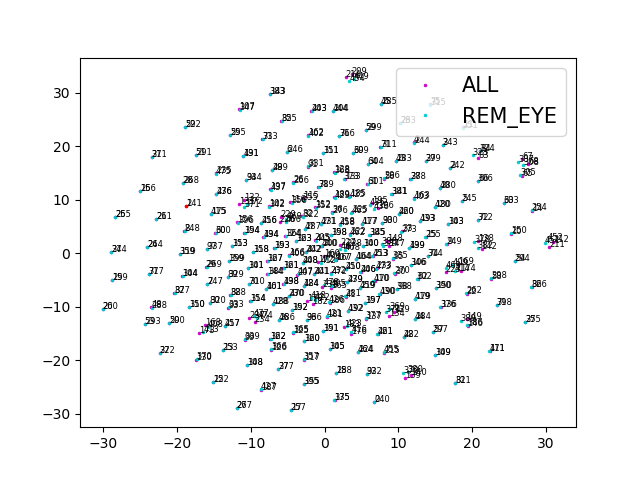
\includegraphics[width=180mm]{t_sne_CAE_hwf_80_weight_all.png}
		\caption{すべてのパーツを使った重み+目抜き画像}
	\end{figure}
	
	\begin{figure}[h]
		\hspace{30mm}
		\centering
		
\includegraphics[width=100mm]{1-2.png}
		\caption{赤の点の画像}
	\end{figure}
	
	AE に目抜き画像を通すと元画像が復元(入力を覚えている?)され,CAE に目抜き画像を通すと目抜き画像が復元する.
	
	\begin{figure}[t]
		\centering
		\begin{subfigure}{0.49\columnwidth}
			\centering
			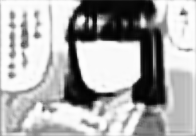
\includegraphics[width=80mm]{CAE_weight_all_10.png}
			\caption{CAE による目抜き画像の出力}
		\end{subfigure}
		\begin{subfigure}{0.49\columnwidth}
			\centering
			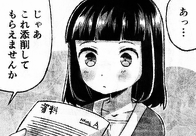
\includegraphics[width=80mm]{AE_weight_all_10.png}
			\caption{AE による目抜き画像の出力}
			\label{fig:AE_decoded}
		\end{subfigure}
	\end{figure}

	このモデルをそのまま用いて目を検出することは難しそう
	
	→明確にパーツを抜いたことを考慮する損失関数を組み込んだモデル構造の作成
\newpage
\section{来週の予定}
	画像の次元圧縮による識別率変化の確認(フィルタサイズを変えながら)

\section{データ補強に関して}
	\begin{itemize}
		\item レイヤがどの人物のものか取り出すことが不可能→命名規則の統一
		\item 曖昧なレイヤの排除
	\end{itemize}

	\begin{figure}[t!]
		\hspace{40mm}
		\centering
		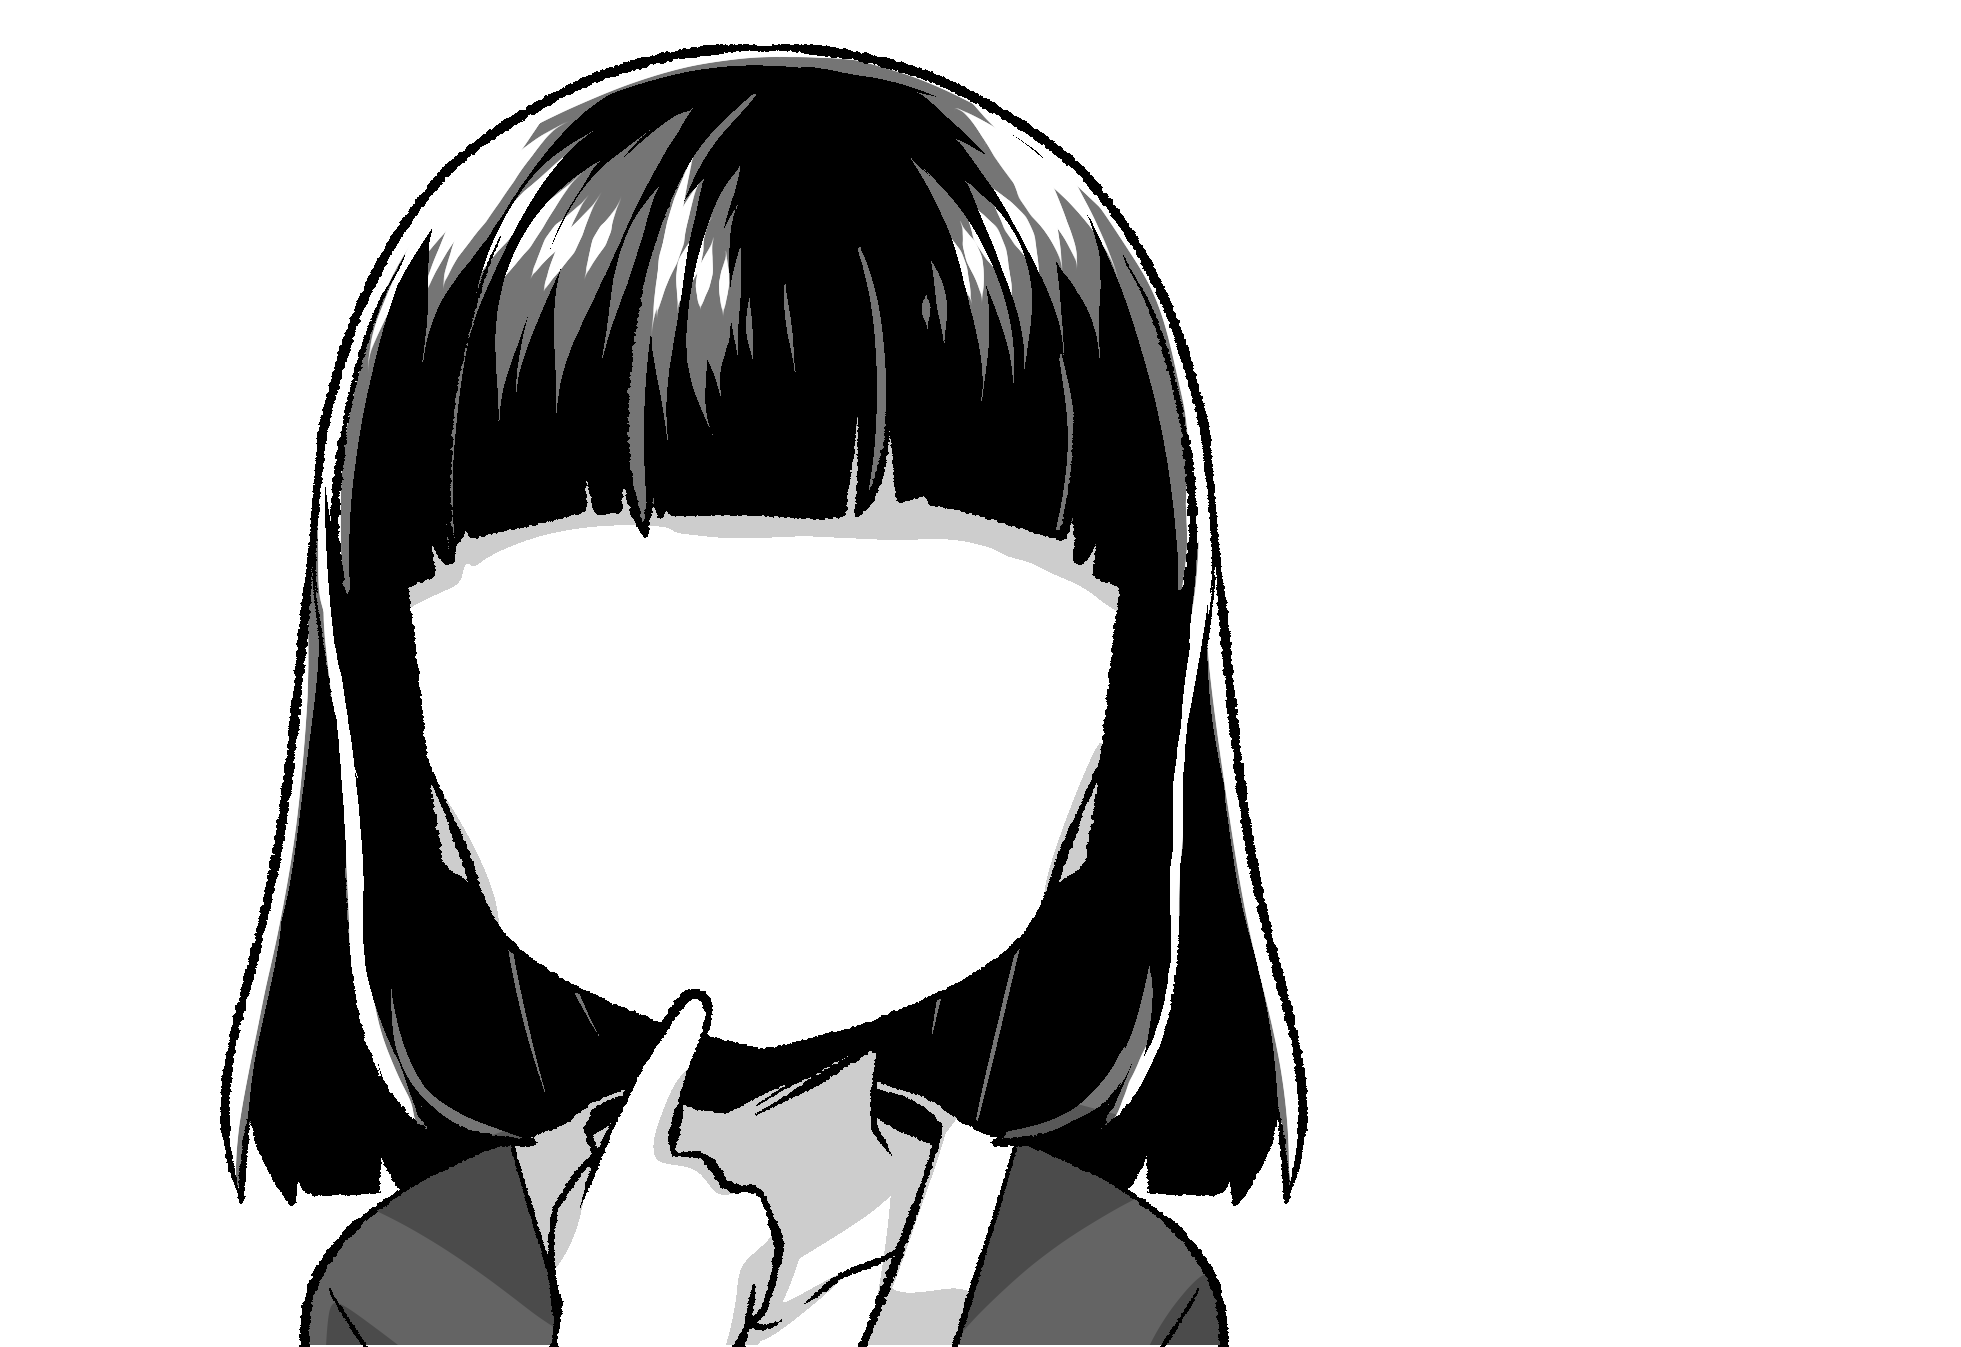
\includegraphics[width=100mm]{学術利用4コマ_萌えタッチ_001_19_身体B-crop_1-2.png}
		\caption{レイヤ名:萌えタッチ\_001\_19\_身体B}
		
		\hspace{40mm}
		\centering
		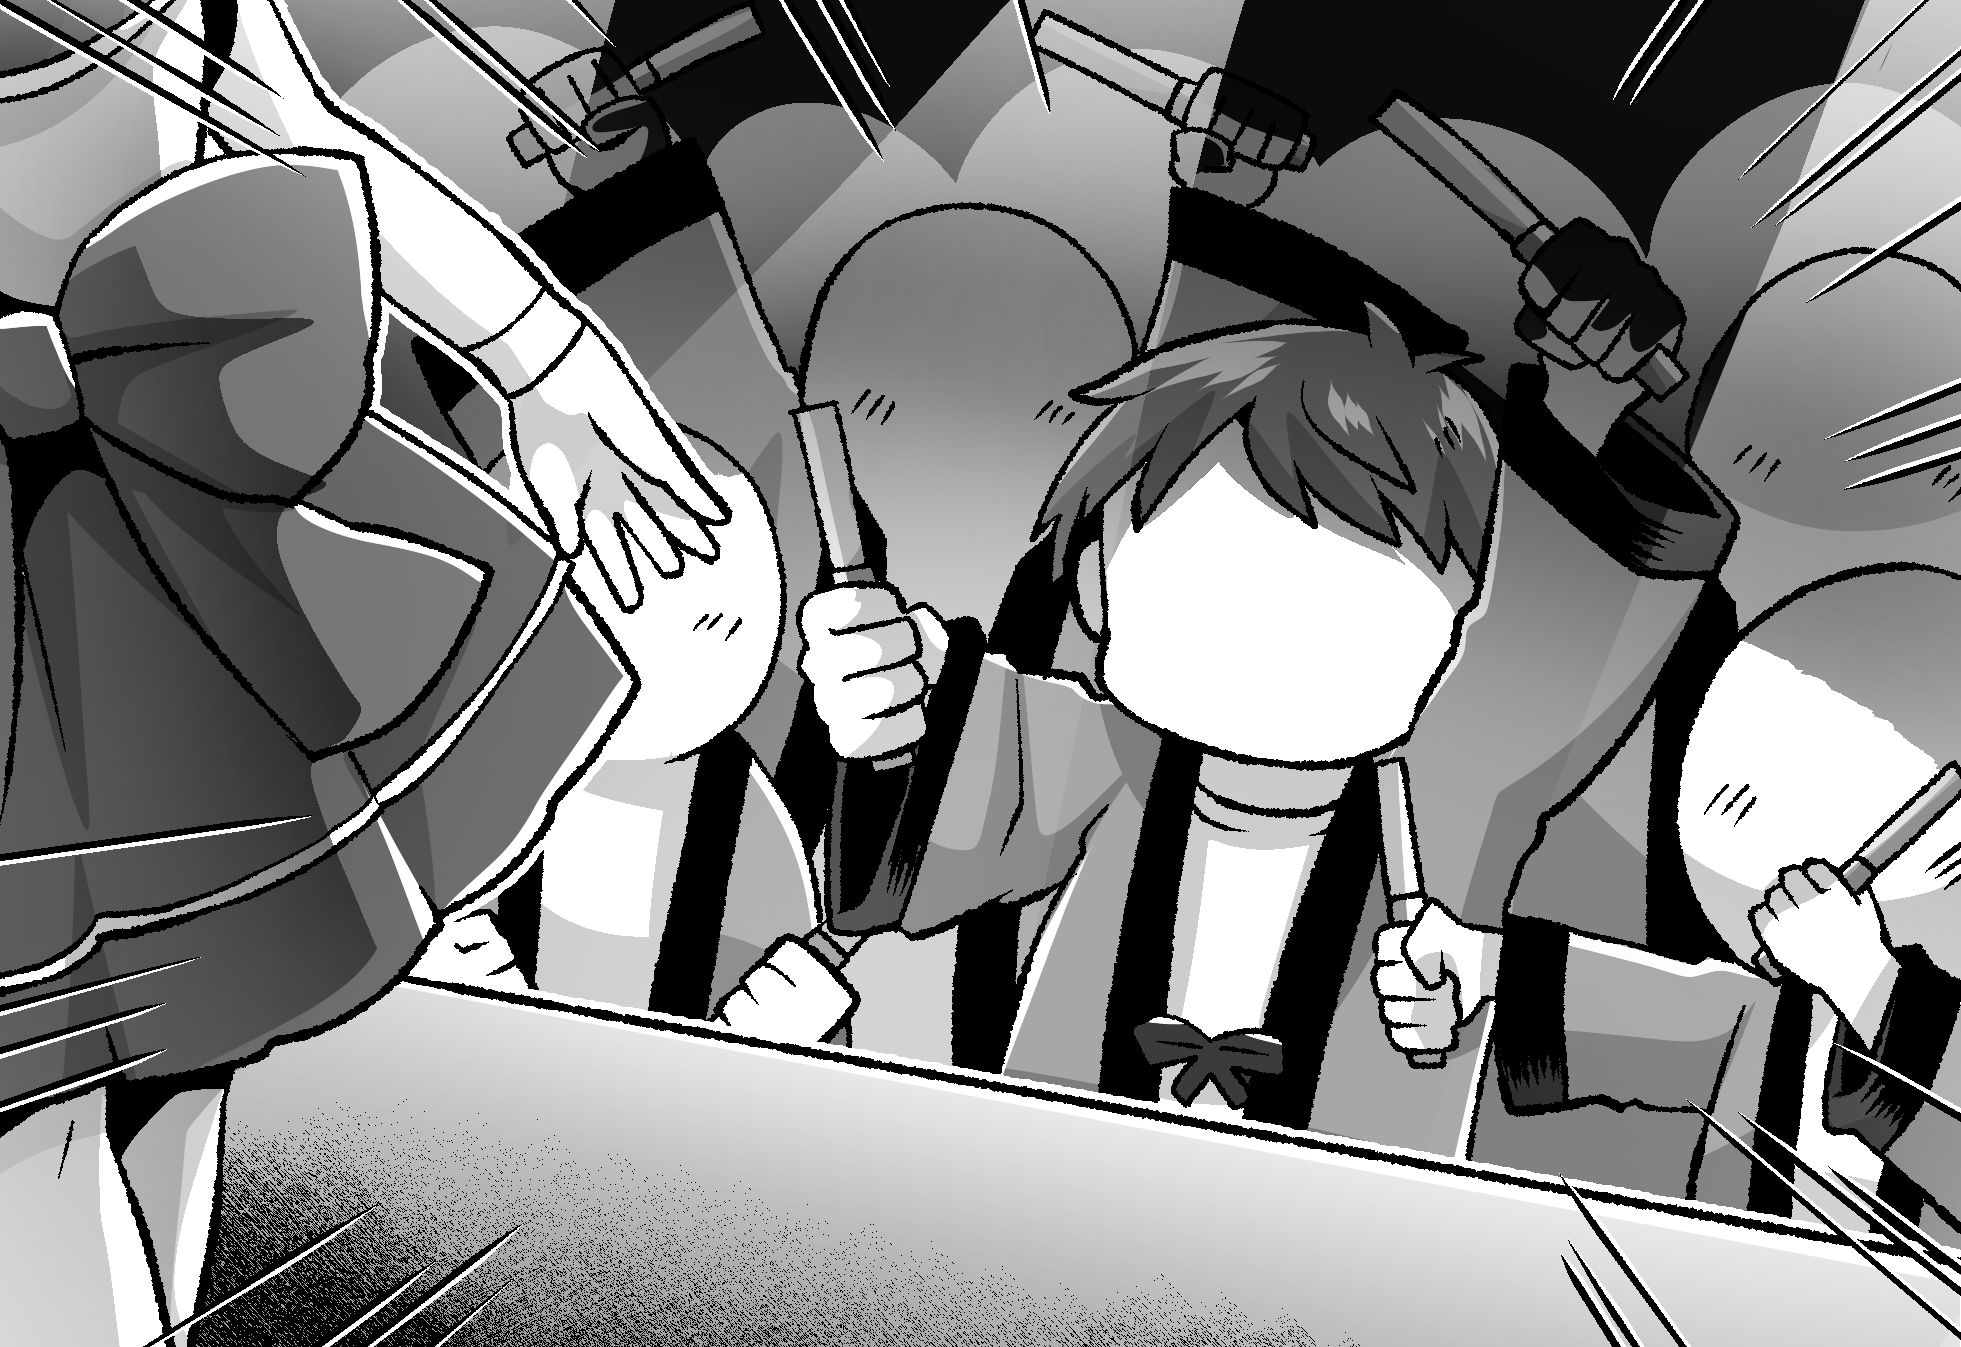
\includegraphics[width=100mm]{学術利用4コマ_萌えタッチ_001_29_身体A-crop_1-4.png}
		\caption{レイヤ名:萌えタッチ\_001\_29\_身体A}
	\end{figure}


\end{document}